\documentclass[ucs, notheorems, handout]{beamer}

\usetheme[numbers,totalnumbers,nologo]{Statmod}
\usefonttheme[onlymath]{serif}
\setbeamertemplate{navigation symbols}{}

\mode<handout> {
    \usepackage{pgfpages}
    \setbeameroption{show notes}
    \pgfpagesuselayout{2 on 1}[a4paper, border shrink=5mm]
    \setbeamercolor{note page}{bg=white}
    \setbeamercolor{note title}{bg=gray!10}
    \setbeamercolor{note date}{fg=gray!10}
}

\usepackage[utf8x]{inputenc}
\usepackage[T2A]{fontenc}
\usepackage[russian]{babel}
\usepackage{tikz}
\usepackage{ragged2e}
\usepackage{wrapfig}
\usepackage{graphicx}
\graphicspath{ {images/} }


\newtheorem{theorem}{Теорема}

\newcommand{\rank}{\mathsf{rank}\ }
\newcommand{\Lrank}{\mathsf{rank}_L\ }
\newcommand{\T}{\mathcal{T}}
\newcommand{\F}{\mathsf{F}}
\newcommand{\MF}{\vec{\F}}
\newcommand{\sfS}{\mathsf{S}}
\newcommand{\sfR}{\mathsf{R}}
\newcommand{\MS}{\vec{\sfS}}
\newcommand{\MSE}{\mathsf{MSE}}
\newcommand{\SSA}{\mathsf{SSA}}
\newcommand{\MSSA}{\mathsf{MSSA}}
\newcommand{\ProjSSA}{\mathsf{ProjSSA}}
\newcommand{\mean}{\mathsf{mean}}
\newcommand{\X}{\mathbf{X}}
\newcommand{\wX}{\overset{\wedge}{\X}}


\title[Поддерживающие ряды MSSA]{Исследование условий для поддерживающих временных рядов в MSSA}

\author{Ткаченко Егор Андреевич, гр.19.Б04-мм}

\institute[Санкт-Петербургский Государственный Университет]{%
    \small
    Санкт-Петербургский государственный университет\\
    Прикладная математика и информатика\\
    Вычислительная стохастика и статистические модели\\
    \vspace{1.25cm}
    Отчет по производственной практике (семестр 6)}

\date[Зачет]{Санкт-Петербург, 2022}

\subject{Talks}

\begin{document}

\begin{frame}[plain]
    \titlepage

    \note{Научный руководитель  к.ф.-м.н., доцент Голяндина Нина Эдуардовна,\\
    кафедра статистического моделирования}
\end{frame}


%\section{Короткая тема}
%\subsection{Общие слова}

\setbeameroption{show notes}
% \setbeameroption{hide notes}

\begin{frame}{Введение}
    Существует задача прогноза временного ряда. При построении прогноза ряда можно использовать другие ряды.

    Цель работы --- выяснить, какие ряды могут улучшить прогноз.
    
    % \cite[Singular Spectrum Analysis with R]{SSA_with_R}
    \note{
        Строить прогнозы очень полезно. Прогноз временных рядов может использоваться в прогнозе погоды, приливов, спроса на товары и многом другом.
         
        По книге \cite[Singular Spectrum Analysis with R]{SSA_with_R} был изучен базовый $\SSA$, разложение рядов, заполнение пропусков в данных, прогноз и базовый $\MSSA$. Для работы с временными рядами и их прогнозом использовался пакет Rssa. Проведены эксперименты с простейшими моделями сигналов для изучения связи между согласованностью сигналов и поддерживающими рядами. 
        Исследовано, при каких отклонениях, сигналы с одинаковой структурой перестают быть согласованными. Проведено сравнение линейных рядов и их аппроксимаций экспонентой как поддерживающих рядов для линейных.
    }
\end{frame}




\begin{frame}
    \frametitle{Базовые определения}
    \begin{block}{Временной ряд}
        Вещественный временной ряд длины $N$:
        $$\F = (f_1, \dots, f_{N}),\ f_j \in \mathbb{R}.$$
    \end{block}

    \begin{block}{Многомерный временной ряд}
        Многомерный временной ряд $\MF$ --- набор $s$ временных рядов $\F^{(p)}$ длин~$N_p$:
        $$\MF = \{\F^{(p)} = (f^{(p)}_1, \dots, f^{(p)}_{N_p}),\ p=1, \dots, s\}.$$
    \end{block}
\end{frame}

\begin{frame}
    \frametitle{Определения}
    \begin{block}{Траекторная матрица}
        $L$-Траекторная матрица ряда $\F$:
        $$\T_{\SSA}(\F) =
        \begin{pmatrix}
            f_1     & f_2    & \dots  & f_{K} \\
            f_2     & f_3    & \dots  & f_{K+1}     \\
            \vdots  & \vdots & \ddots & \vdots  \\
            f_{L} & f_{L+1}    & \dots  & f_{N} \\
        \end{pmatrix}.$$
        для многомерного ряда $\MF$:
        $$\T_{\MSSA}(\MF) = [\T_{\SSA}(\F^{(1)}): \dotso :\T_{\SSA}(\F^{(s)})].$$\\
        Из траекторной матрицы можно восстановить ряд.
    \end{block}

    
\end{frame}

\begin{frame}
    \begin{block}{$L$-Ранг ряда}
        $L$-Ранг ряда --- это ранг его траекторной матрицы: $$r_p =\Lrank \F = \rank \T_{\SSA}(\F),\qquad \Lrank \MF = \rank \T_{\MSSA}(\MF).$$
    \end{block}


    \begin{block}{Ранг ряда}
        Ряд называется рядом конечного ранга $r$, если его $L$-ранг равен $r$ для любой длины окна $L$ и любой достаточно большой длины $N$.
    \end{block}
\end{frame}


\begin{frame}{Алгоритмы SSA и MSSA для аппроксимации рядом ранга $r$}
    \structure{\textbf{Вход:}}
    Ряд $\mathsf{F_1}$ для SSA или многомерный ряд $\mathsf{F}$ для MSSA;\\
    длина окна $L \leq N_1$ для SSA или $L \leq N_p$ для MSSA;\\
    ранг аппроксимирующего ряда r.\\
    
    \begin{block}{Алгоритм}
        \begin{enumerate}
            \item Вложение. Временной ряд переводится в L-траекторную матрицу $\X$
            \item Сингулярное разложение. Методом SVD матрица $\X$ раскладывается на сумму $d$ матриц $\X_i$ ранга 1.
            % \item Группировка. Множество индексов $\{1, \dots, d\}$ делится на $m$ непересекающихся множеств $I_1 ,\dots, I_m$. Матрицы $\X_i$ суммируются в $m$ матриц $\X_{I_j}$
            \item Группировка. Первые $r$ матрицы $\X_i$ суммируются.
            \item Восстановление. Полученная сумма матриц диагональным усреднением восстанавливаются в ряд.
        \end{enumerate}
        
        % \begin{enumerate}
        %     \item[1] Получение L-траекторной матрицы $\mathbf{X}$ временного ряда:\\
        %         $\mathbf{X} = \mathcal{T}_{SSA}(\mathsf{F_1})$ для SSA или $\mathbf{X} = \mathcal{T}_{MSSA}(\mathsf{F})$ для MSSA.
        %     \item[2] Методом SVD матрица $\mathbf{X}$ раскладывается на сумму $d$ матриц $\mathbf{X}_i$ ранга 1, где: $d = \mathsf{rank}\ \mathbf{X}$.
        %     % $\mathbf{X}_i = \sqrt{\lambda_i}U_iV_i^T$, где: $d = \mathsf{rank}\ \mathbf{X}$;\\
        %     % $\lambda_i$ --- собственные числа матрицы $\mathbf{XX}^T$ ($\lambda_1 \geq \dotso \geq \lambda_L \geq 0$);\\
        %     % $U_i$ --- собственные вектора матрицы $\mathbf{XX}^T$; $V_i = \mathbf{X}^T U_i / \sqrt{\lambda_i}$.\\
        %     \item[3] Первые $r$ матриц $\mathbf{X}_i$ складываются и восстанавливаются в ряд (SSA) или многомерный ряд (MSSA)
        % \end{enumerate}
    \end{block}
    
    \structure{\textbf{Выход:}}
    % Разложение исходного ряда на сумму $m$ рядов.
    Аппроксимирующий ряд конечного ранга r.

\end{frame}

\begin{frame}
    \begin{block}{Линейная рекуррентная формула; управляемый ЛРФ ряд}
        % ЛРФ --- формула, выражающая каждый член последовательности через линейную комбинацию предыдущих членов.\\
        Ряд $\mathsf{F_p} = (f_i)_{i=1}^{N_p}$ --- управляемый ЛРФ, если существуют такие $a_1, \dotso, a_d$, что:
        $$f_{i+d} = \sum_{k=1}^d a_k f_{i+d-k},\ 1 \leq i \leq N_p - d,\ a_d \neq 0,\ d < N_p - 1.$$
    \end{block}

    % \begin{block}{Замечание}
    %     Ряд конечного ранга является управляемым ЛРФ.
    % \end{block}
    
    \begin{block}{Прогноз ряда}
        Прогноз вещественного временного ряда $\mathsf{F}_p$:
        $$\overset{\sim}{\mathsf{f}}_{N_p} = \sum_{k=1}^{L-1} a_k f_{N_p-k}.$$
        % $$\overset{\sim}{\mathsf{f}}_{N_p} = (\overset{\sim}{f}_{N_p}, \dots, \overset{\sim}{f}_{N_p + \overset{\sim}{N}_p - 1}), \overset{\sim}{f_j} \in \mathbb{R}.$$
    \end{block}

    % \begin{block}{Коэффициенты ЛРФ $a_1, \dotso, a_{L-1}$}
    %     $$(a_1, \dotso, a_{L-1}) = \mathcal{R}_L=\frac{1}{1-\sum_{j=1}^r \pi(U_j)^2} \sum_{j=1}^r \pi(U_j) \underline{U_j},$$
    %     где $\pi(U_j)$ --- последняя координата вектора $U_j$,\\ $\underline{U_j}$ --- вектор $U_j$ без последней координаты.
    % \end{block}
    \note{
        ЛРФ позволяет прогнозировать ряд на одно значение, а поэтому на любое количесвто значений.
    }
\end{frame}

\begin{frame}
    \frametitle{Задача}

    Пусть имеется временной ряд $\mathsf{F_1 = S_1 + R_1}$, где
    \begin{itemize}
        \item Сигнал $\mathsf{S_1}$ --- ряд управляемый ЛРФ.
        \item Шум $\mathsf{R_1}$ --- ряд без структуры.
    \end{itemize} 

    \structure{\textbf{Задача:}}
    спрогнозировать сигнал $\mathsf{S_1}$.

    Пусть помимо ряда $\mathsf{F_1}$ имеется временной ряд $\mathsf{F_2}$.

    \structure{\textbf{Идея:}}
    использование ряда $\mathsf{F_2}$ может улучшить прогноз сигнала $\mathsf{S_1}$.

    \begin{itemize}
        \item Второй ряд дает алгоритму больше данных, которые могут улучшить ЛРФ.
        \item Второй ряд может сделать прогноз хуже, если его структура отличается от первого.
    \end{itemize}
\end{frame}

\begin{frame}
    \begin{block}{Ошибка прогноза $\overset{\sim}{\mathsf{S}}$ сигнала $\mathsf{S_1}$}
        $\mathsf{MSE(\overset{\sim}{S}, S_1)} = \frac{1}{N_{f}} \sum_{i = N + 1}^{N + N_{f}} (\overset{\sim}{s}_i - s_i)^2$
    \end{block}

    \begin{block}{Поддерживающий ряд (для прогноза)}
        Ряд $F_2$ --- поддерживающий, если $\mathsf{MSE(\overset{\sim}{S}_{MSSA}, S_1)} < \mathsf{MSE(\overset{\sim}{S}_{SSA}, S_1)}$
    \end{block}

    \structure{\textbf{Вопрос:}} Как понять, что ряд поддерживающий? 

    \begin{block}{Согласованность}
        \begin{itemize}
            \item Сигналы $\mathsf{S_1, S_2}$ полностью согласованы, если $r_{MSSA} = r_1 = r_2$
            \item Сигналы $\mathsf{S_1, S_2}$ полностью не согласованы, если $r_{MSSA} = r_1 + r_2$
        \end{itemize}
    \end{block}
\end{frame}

\begin{frame}

    \begin{block}{Относительная ошибка}
        Относительная ошибка прогноза (восстановления)
        $$ error_{rel} = \frac{error_{\SSA} - error_{\MSSA}}{error_{\SSA} + error_{\MSSA}},$$ где $error_{\SSA}, error_{\MSSA}$ --- ошибки прогноза (восстановления) методами $\SSA$ и $\MSSA$ соответственно.
    \end{block}
    

    Как интерпретировать значения относительной ошибки? 
    \begin{itemize}
        \item значения больше $0$ значат, что что $\MSSA$ лучше $\SSA$;
        \item значения меньше $0$ значат, что что $\MSSA$ хуже $\SSA$;
        \item значения около $0$ значат что ошибки примерно равны;
        \item значения далеко от $0$ значат, что ошибки сильно отличаются.
    \end{itemize}

    \note{
        
    Значения относительной ошибки легко расположить на графике (она принимает значения от -1 до 1). По значению относительной ошибки легче понять, какой метод лучше (не надо сравнивать два значения ошибок, которые просто положительны и могут быть любых порядков). Но относительную ошибку нельзя считать когда $error_{\SSA} = error_{\MSSA} = 0$.

    Как интерпретировать значения относительной ошибки? 
    }

\end{frame}

\begin{frame}{Выбор количества компонент для MSSA}


    \begin{block}{Нормирование сигналов}
        Все сигналы в этом и следующих экспериментах будут нормироваться, чтобы амплитуда сигнала не влияла на ошибки прогноза и восстановления. Например, для косинуса: $s_j^{(i)} = A \cos(\frac{2\pi j}{T_i})$, где $A$ --- такая константа, что $\mean(|s_j^{(i)}|) = 1$.
    \end{block}

    \begin{block}{Структура рядов}
        Первый ряд --- простой сигнал, зависящий от параметра с аддитивным гауссовым шумом с дисперсией $\sigma_1^2 = 0.2^2$.
        Второй ряд --- сигналом того же вида, с несколько отличающимся параметром и без шума.
    \end{block}

    \note{
        Когда сигналы похожи, их можно считать согласованными и лучше использовать (при прогнозе или восстановлении сигнала) ранг равный рангу одного сигнала. Когда сигналы отличаются, их следует считать не согласованными и использовать ранг равный сумме рангов сигналов.

        Будет ли ошибка $\MSSA$ меньше при таком выборе ранга для алгоритма $\MSSA$ в восстановлении и прогнозе первого ряда. И будут ли при этом вторые ряды поддерживающими.

        По определению, когда сигналы похожи, их можно считать согласованными и лучше использовать (при прогнозе или восстановлении сигнала) ранг равный рангу одного сигнала. Когда сигналы отличаются, их следует считать не согласованными и использовать ранг равный сумме рангов сигналов. Исследуем, будет ли ошибка $\MSSA$ меньше при таком выборе ранга для алгоритма $\MSSA$ в восстановлении и прогнозе первого ряда. И будут ли при этом вторые ряды поддерживающими.

        Выберем в качестве первого ряда простой сигнал, зависящий от параметра (например, у косинуса параметр --- период) с аддитивным гауссовым шумом с дисперсией $\sigma_1^2 = 0.2^2$.
        Второй ряд будет простым сигналом того же вида, с несколько отличающимся параметром и без шума.
        Восстановим и спрогнозируем первый ряд с помощью $\SSA$, $\MSSA$ считая ряды согласованными и $\MSSA$ считая ряды несогласованными.
}

\end{frame}

\begin{frame}{Относительные ошибки для косинуса}
    \begin{wrapfigure}{r}{6.5cm}
        \vspace{-4\intextsep}
        \centering
        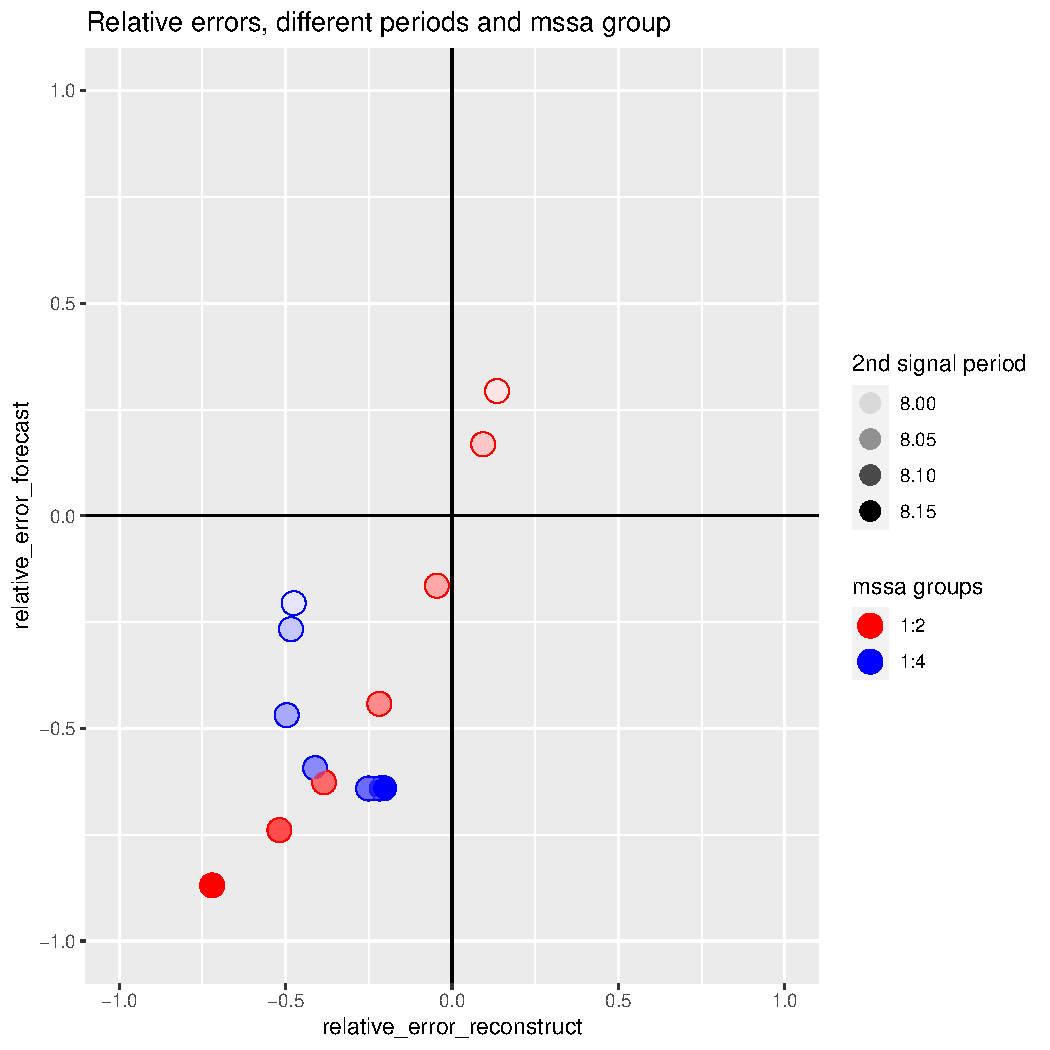
\includegraphics[width=0.7\textwidth]{experiment_1_cos.pdf}
    \end{wrapfigure}

    Функция для сигналов --- $s^{(i)}_j = A \cos(\frac{2\pi j}{T_i})$.
    Сигнал $\sfS^{(1)}$ --- косинус с периодом $T_1 = 8$.
    Сигналы $\sfS^{(2)}$ --- косинусы с периодами $T_2 \in \{8$, $8.02$, $8.04$, $8.06$, $8.08$, $8.1$, $8.15\}$.
    Длина ряда $N = 100$, длина прогноза $N_{for} = 20$.

    \note{
        Функция для сигналов --- $s^{(i)}_j = A \cos(\frac{2\pi j}{T_i})$.
        Сигнал $\sfS^{(1)}$ --- косинус с периодом $T_1 = 8$.
        Сигналы $\sfS^{(2)}$ --- косинусы с периодами $T_2 \in \{8$, $8.02$, $8.04$, $8.06$, $8.08$, $8.1$, $8.15\}$.

        Ранг косинуса равен 2, поэтому для $\MSSA$ используются первые 2 или первые 4 компоненты разложения, а для $\SSA$ только 2.

        На графике видим, что с увеличением разницы периодов рядов использование четырех компонент становится лучше и для прогноза и для восстановления сигнала, но при этом второй ряд является поддерживающим только для случаев, когда второй сигнал совпадает с первым или очень близок к нему, а ранг для $\MSSA$ 2.
    }
\end{frame}

\begin{frame}{Относительные ошибки для экспоненты}
    \begin{wrapfigure}{r}{6.5cm}
        \vspace{-4\intextsep}
        \centering
        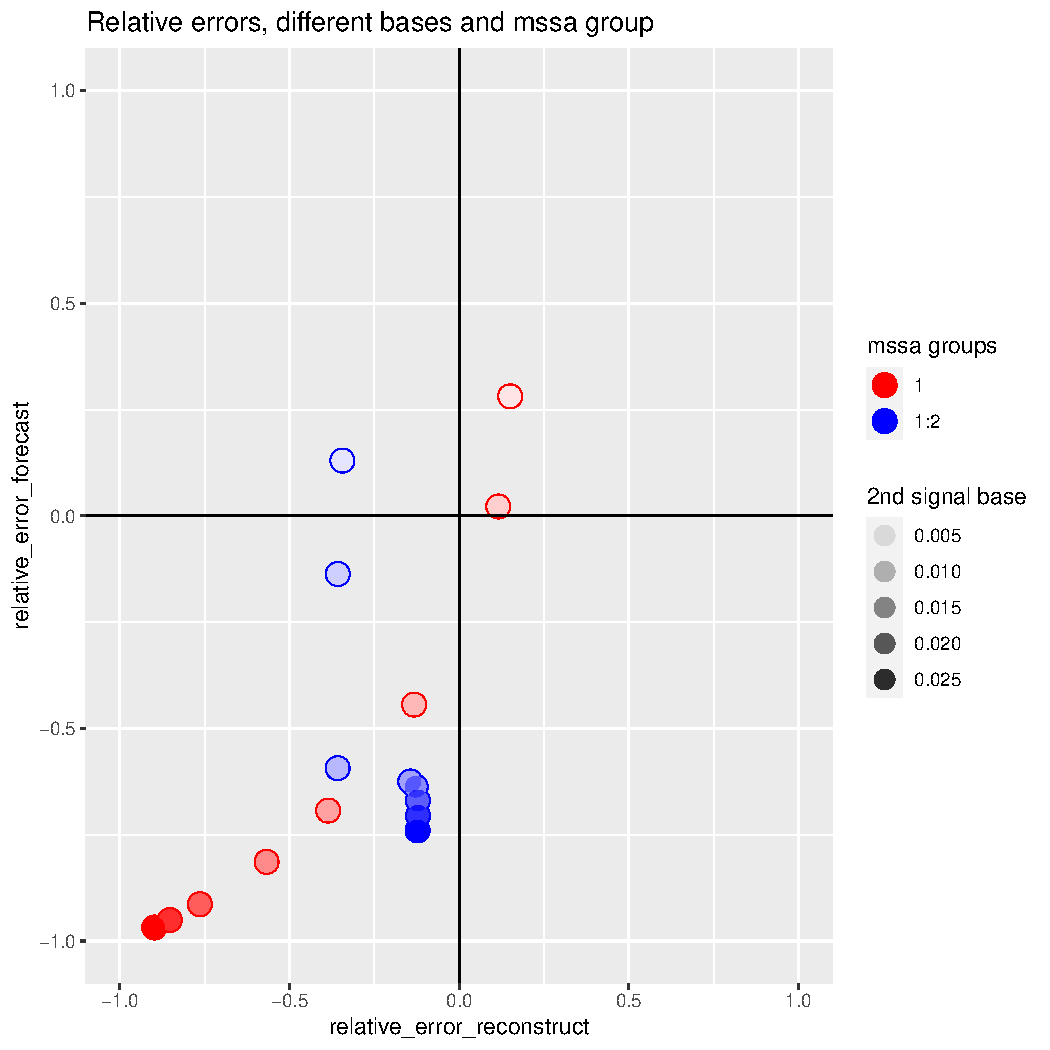
\includegraphics[width=0.7\textwidth]{experiment_1_exp.pdf}
    \end{wrapfigure}

    Функция для сигналов --- $s^{(i)}_j = A \exp(j\lambda_i)$.
    Сигнал $\sfS^{(1)}$ --- экспонента c $\lambda_1 = 0.005$.
    Сигналы $\sfS^{(2)}$ --- экспонента c $\lambda_2 \in \{0.005$, $0.0075$, $0.01$, $0.0125$, $0.015$, $0.02$, $0.025$, $0.03\}$.
    Длина ряда $N = 100$, длина прогноза $N_{for} = 20$.

    \note{
        Функция для сигналов --- $s^{(i)}_j = A \exp(j\lambda_i)$.
        Сигнал $\sfS^{(1)}$ --- нормированная показательная функция c $\lambda_1 = 0.005$.
        Сигналы $\sfS^{(2)}$ --- нормированная показательная функция c $\lambda_2 \in \{0.005$, $0.0075$, $0.01$, $0.0125$, $0.015$, $0.02$, $0.025$, $0.03\}$.

        Ранг показательной функции равен 1, поэтому для $\MSSA$ используется первая или первые 2 компоненты разложения, а для $\SSA$ только первая.

        На графике видим похожий результат: с отдалением $\lambda_2$ от $\lambda_1$ использование двух компонент становится лучше. Второй ряд поддерживающий только для случаев, когда он равен первому или очень близок к нему, но на этот раз не только когда ранг для алгоритма $\MSSA$ равен рангу ряда.
    }
\end{frame}

\begin{frame}{Относительные ошибки для косинуса с модуляцией ($T = const$)}
    \begin{wrapfigure}{r}{6.5cm}
        \vspace{-4\intextsep}
        \centering
        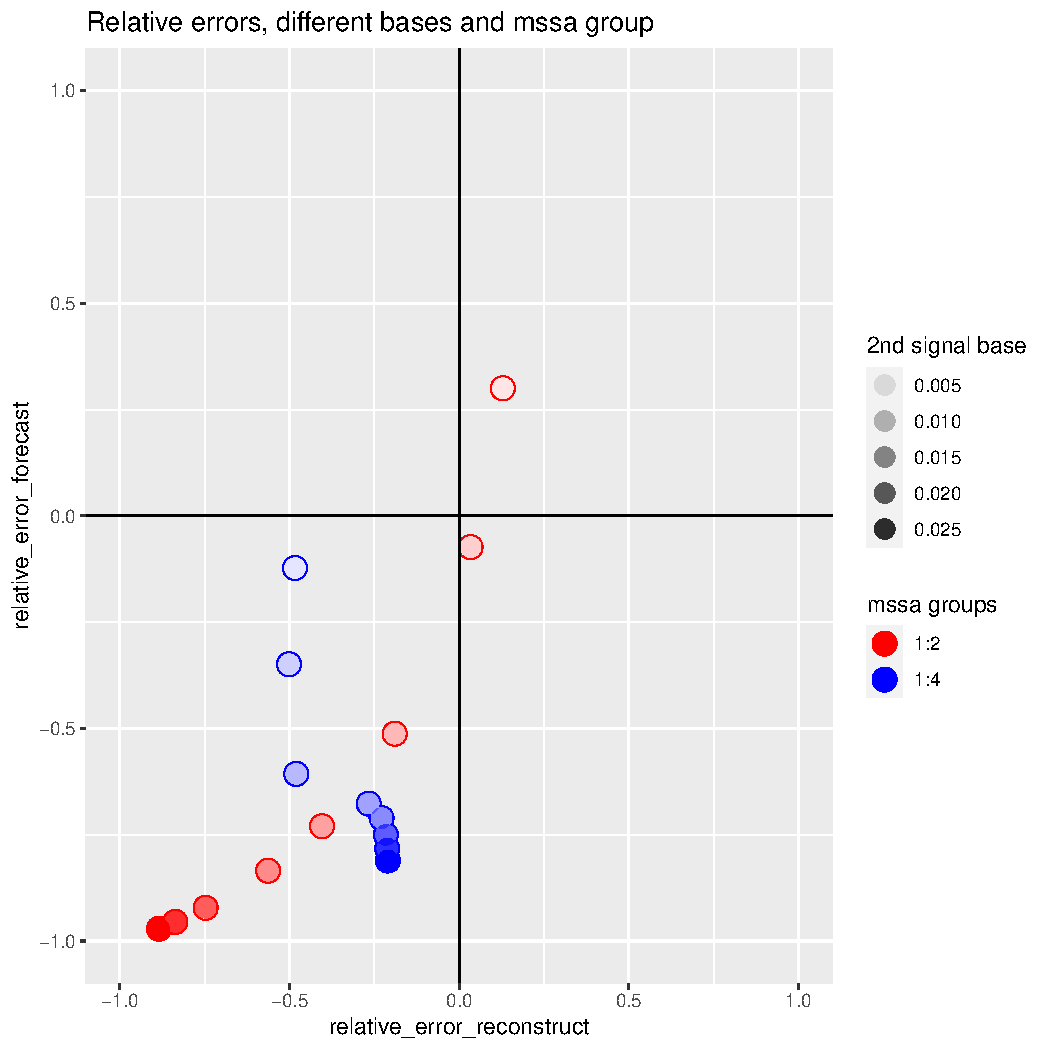
\includegraphics[width=0.7\textwidth]{experiment_1_expcos1.pdf}
    \end{wrapfigure}
    Функция для сигналов --- $s^{(i)}_j = A \exp(j\lambda_i) \cos(\frac{2\pi j}{8})$.
    Сигнал $\sfS^{(1)}$ --- функция c $\lambda_1 = 0.005$.
    Сигналы $\sfS^{(2)}$ --- функция c $\lambda_2 \in \{0.005$, $0.0075$, $0.01$, $0.0125$, $0.015$, $0.02$, $0.025$, $0.03\}$.
    Длина ряда $N = 100$, длина прогноза $N_{for} = 20$.

    \note{
        Функция для сигналов --- $s^{(i)}_j = A \exp(j\lambda_i) \cos(\frac{2\pi j}{8})$.
        Сигнал $\sfS^{(1)}$ --- функция c $\lambda_1 = 0.005$.
        Сигналы $\sfS^{(2)}$ --- функция c $\lambda_2 \in \{0.005$, $0.0075$, $0.01$, $0.0125$, $0.015$, $0.02$, $0.025$, $0.03\}$.

        Ранг косинуса с модуляцией равен 2, поэтому для $\MSSA$ используются первые 2 или первые 4 компоненты разложения, а для $\SSA$ только 2.

        На графике видим аналогичный результат для косинусов с модуляцией при изменении модулирующей функции.
    }
\end{frame}

\begin{frame}{Относительные ошибки для косинуса с модуляцией ($\lambda = const$)}
    \begin{wrapfigure}{r}{6.5cm}
        \vspace{-4\intextsep}
        \centering
        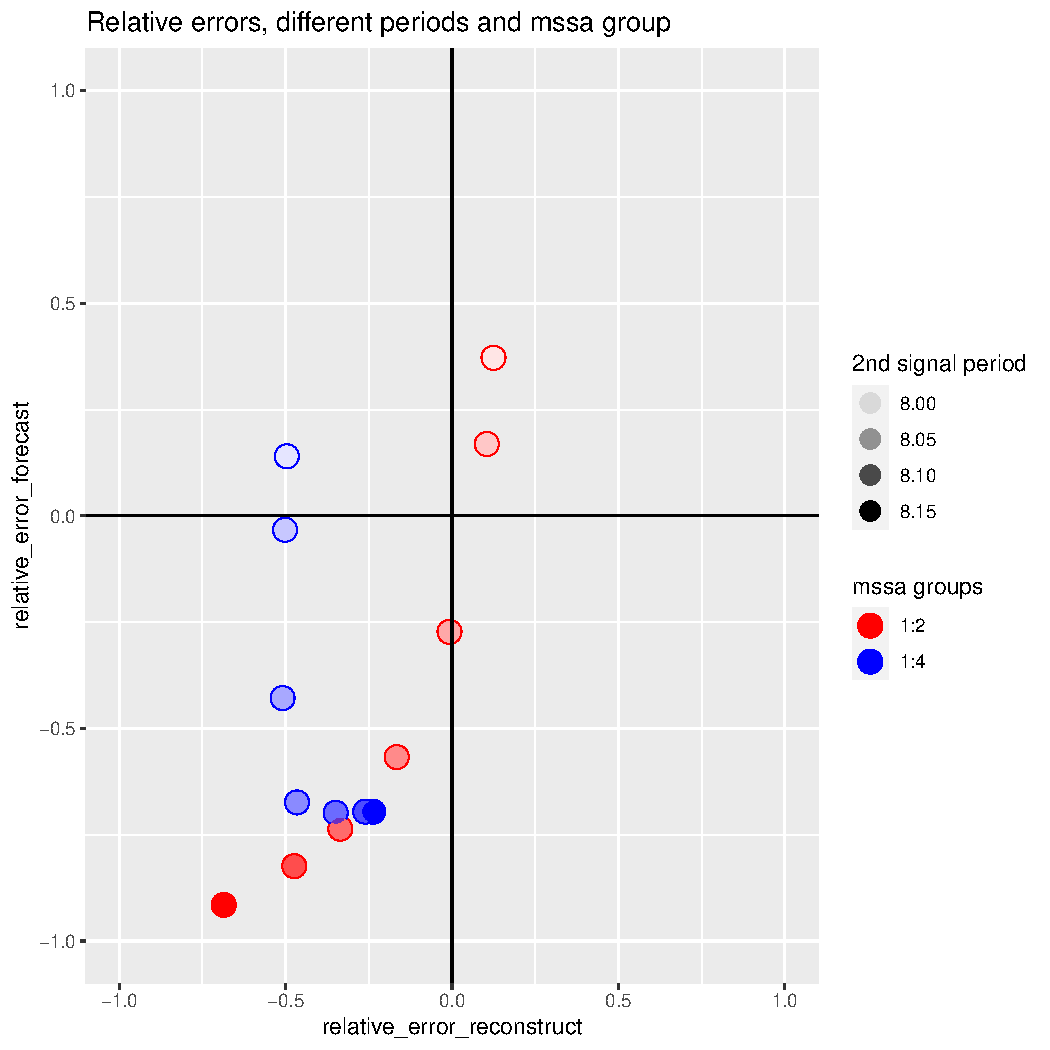
\includegraphics[width=0.7\textwidth]{experiment_1_expcos2.pdf}
    \end{wrapfigure}
    Функция для сигналов --- $s^{(i)}_j = A \exp(0.02j) \cos(\frac{2\pi j}{T_i})$.
    Сигнал $\sfS^{(1)}$ --- функция c $T_1 = 8$.
    Сигналы $\sfS^{(2)}$ --- функция c $T_2 \in \{8$, $8.02$, $8.04$, $8.06$, $8.08$, $8.1$, $8.15\}$.
    Длина ряда $N = 100$, длина прогноза $N_{for} = 20$.

    \note{
        Функция для сигналов --- $s^{(i)}_j = A \exp(0.02j) \cos(\frac{2\pi j}{T_i})$.
        Сигнал $\sfS^{(1)}$ --- функция c $T_1 = 8$.
        Сигналы $\sfS^{(2)}$ --- функция c $T_2 \in \{8$, $8.02$, $8.04$, $8.06$, $8.08$, $8.1$, $8.15\}$.

        Ранг косинуса с модуляцией равен 2, поэтому для $\MSSA$ используются первые 2 или первые 4 компоненты разложения, а для $\SSA$ только 2.

        На графике видим аналогичный результат для косинусов с модуляцией при изменении модулирующей функции.
    }
\end{frame}

\begin{frame}{Результат первого эксперимента}

    Для всех видов сигналов при отклонении второго сигнала от первого всегда наступал момент, когда использование удвоенного ранга дает меньшие ошибки прогноза и восстановления.

    \note{
        Но при этом, второй ряд редко оказывался поддерживающим, потому что большая часть наблюдений находилась в нижней левой четверти.
    }
    
\end{frame}

\begin{frame}{Ошибки прогноза для разных шумов первого ряда и параметров второго ряда}
    
    Гипотеза: при увеличении шума первого ряда, $\MSSA$ станет лучше для любого отклонения второго ряда. Если это так, то можно найти зависимость граничного значения $\sigma_1$ (при котором $\SSA$ становится хуже $\MSSA$) от изменения параметра второго сигнала.



    \note{Никита Федоров в свей выпускной квалификационной работе изучал влияние величины второго шума на результаты работы $\SSA, \MSSA, \ProjSSA$ \cite[глава 3, стр. 17]{supportive_mssa}. Рассмотрим влияние величины первого шума на прогноз $\SSA$ и $\MSSA$, с не зашумленным вторым рядом.

    Как и в первом эксперименте, выберем в качестве первого ряда простой сигнал, зависящий от параметра с аддитивным гауссовым шумом с несколькими значениями дисперсией $\sigma_1^2$.
    Второй ряд будет простым сигналом того же вида, с несколько отличающимся параметром и без шума.
    Спрогнозируем первый ряд с помощью $\SSA$ и $\MSSA$ используя в алгоритме ранг равный рангу сигнала.
    
    Если графики ошибок прогноза $\SSA$ и $\MSSA$ будут пересекаться, то найдем значения $\sigma_1$ при которых это происходит, это и будут граничные значения $\sigma_1$.}
\end{frame}

\begin{frame}{Сигнал косинус}
    \begin{figure}[h]
        \centering
        \begin{minipage}{.5\textwidth}
            \centering
            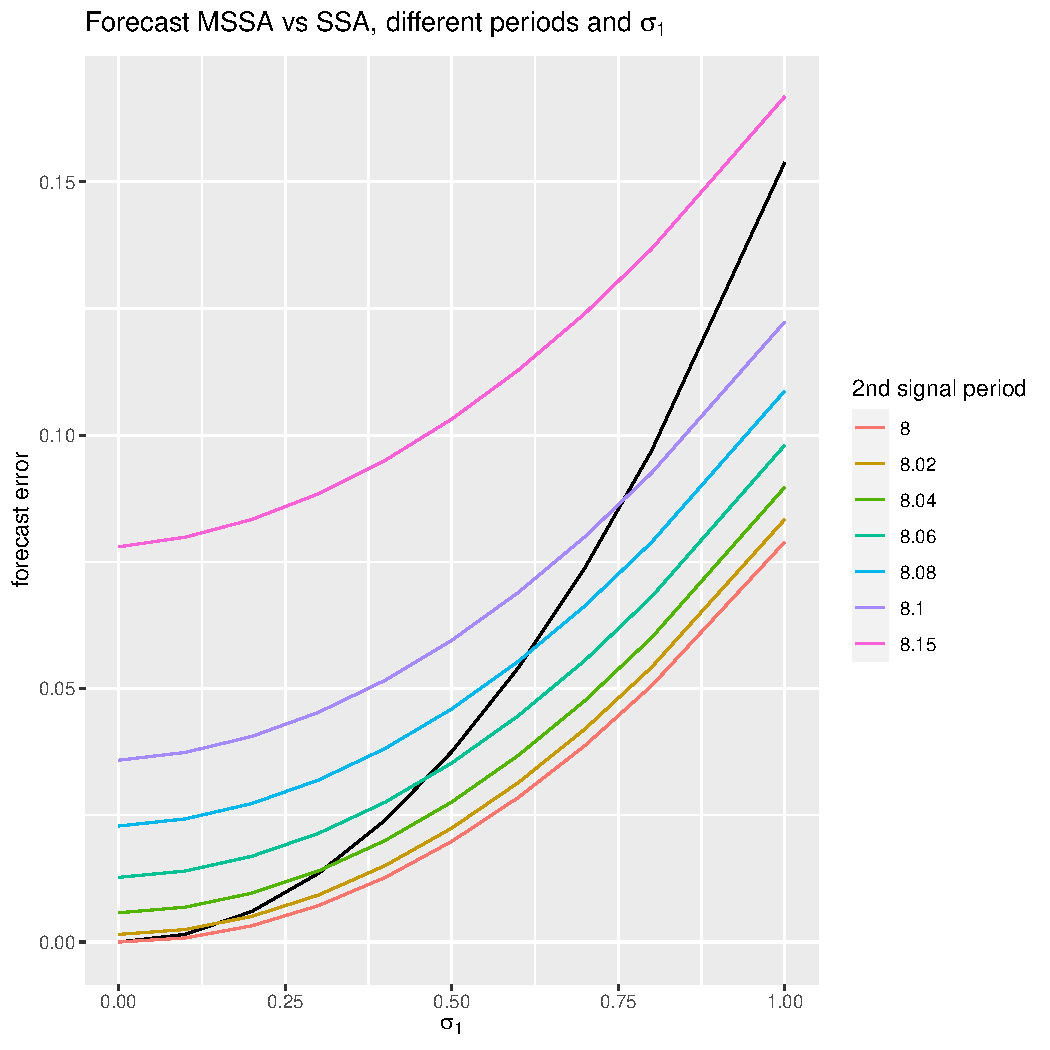
\includegraphics[width=\textwidth]{experiment_2_cos1.pdf}
            % \caption{Ошибка прогноза $\SSA$ и $\MSSA$ для косинусов.}
            % \label{fig:exp2_cos1}
        \end{minipage}%
        \begin{minipage}{.5\textwidth}
            \centering
        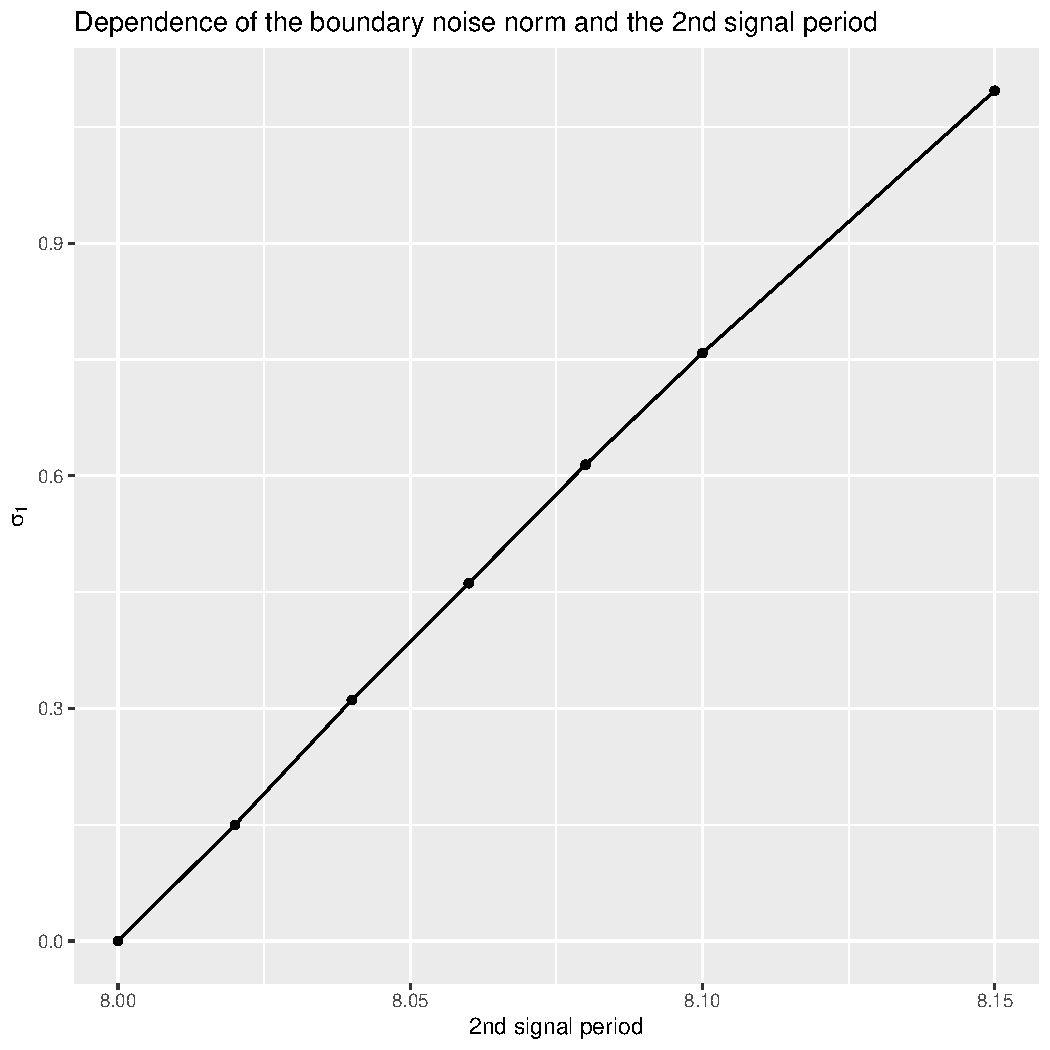
\includegraphics[width=\textwidth]{experiment_2_cos2.pdf}
        % \caption{Зависимость граничного значения $\sigma_1$ от периода второго сигнала}
        % \label{fig:exp2_cos2}
        \end{minipage}
    \end{figure}

    Модель сигнала --- $s_j^{(i)} = A \cos(\frac{2\pi j}{T_i})$. Параметры для сигналов: $T_1 = 8$, $T_2 \in \{8$, $8.02$, $8.04$, $8.06$, $8.08$, $8.1$, $8.15\}$, $\sigma_1 \in \{0, 0.1, 0.2, 0.3, 0.4, 0.5, 0.6, 0.7, 0.8, 1\}$.

    \note{
        

        На левом графике видим, что график ошибки прогноза $\SSA$ (черная линия) пересекает все графики ошибок прогноза $\MSSA$ кроме одного, но они очевидно пересекутся при большем $\sigma_1$. Пересечения графиков будем искать с помощью интерполяции, а для случаев, когда пересечения не было --- с помощью экстраполяции. 

        На на правом графике изображены полученные граничные значения $\sigma_1$ для каждого второго сигнала. Видна линейная зависимость.
    }
\end{frame}

\begin{frame}{Сигнал экспонента}
    \begin{figure}[h]
        \centering
        \begin{minipage}{.5\textwidth}
            \centering
            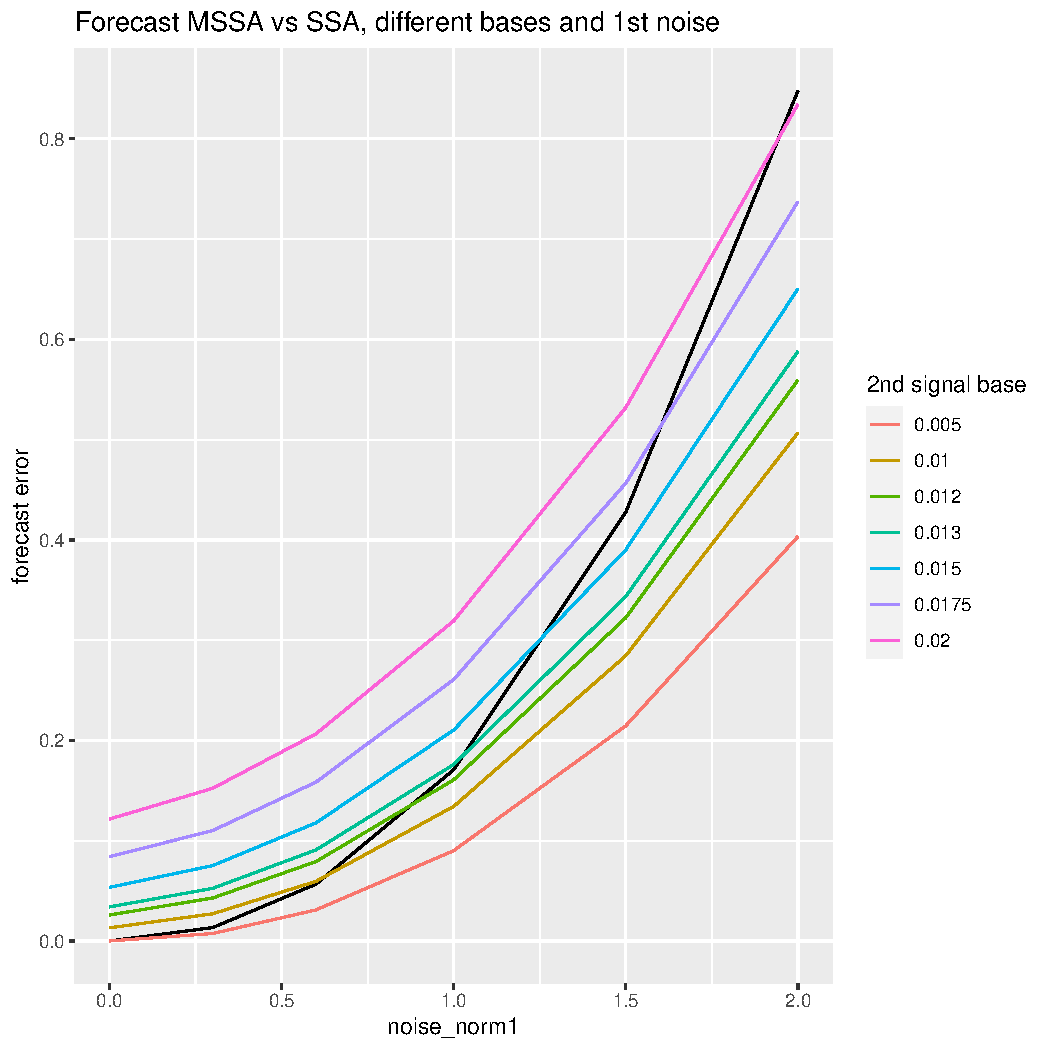
\includegraphics[width=\textwidth]{experiment_2_exp1.pdf}
            % \caption{Ошибка прогноза $\SSA$ и $\MSSA$ для косинусов.}
            % \label{fig:exp2_cos1}
        \end{minipage}%
        \begin{minipage}{.5\textwidth}
            \centering
        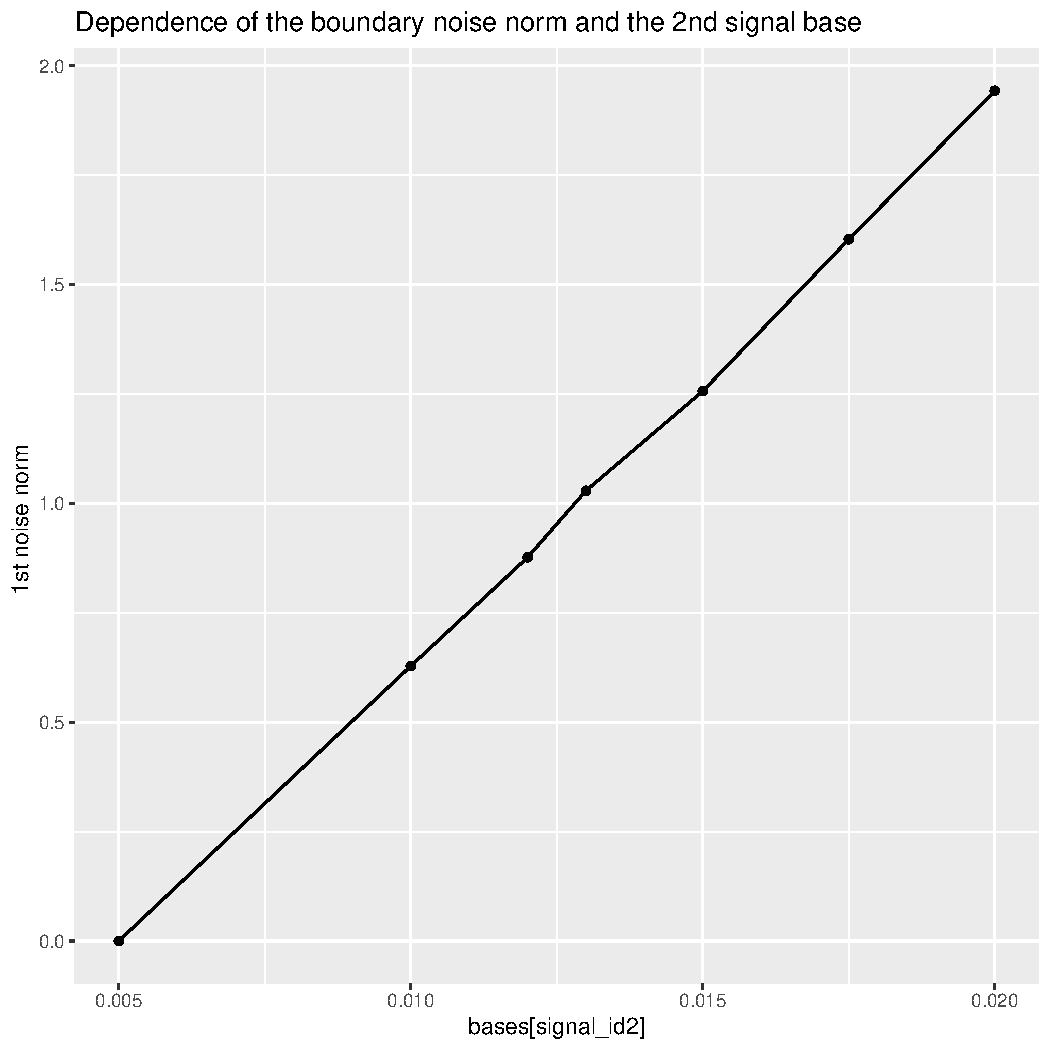
\includegraphics[width=\textwidth]{experiment_2_exp2.pdf}
        % \caption{Зависимость граничного значения $\sigma_1$ от периода второго сигнала}
        % \label{fig:exp2_cos2}
        \end{minipage}
    \end{figure}
    Модель сигнала --- $s^{(i)}_j = A \exp(j\lambda_i)$. Параметры для сигналов: $\lambda_1 = 0.005$, $\lambda_2 \in \{0.005$, $0.01$, $0.012$, $0.013$, $0.015$, $0.0175$, $0.02\}$, $\sigma_1 \in \{0, 0.3, 0.6, 1, 1.5, 2\}$

    \note{
        Модель сигнала --- $s^{(i)}_j = A \exp(j\lambda_i)$. Параметры для сигналов: $\lambda_1 = 0.005$, $\lambda_2 \in \{0.005$, $0.01$, $0.012$, $0.013$, $0.015$, $0.0175$, $0.02\}$, $\sigma_1 \in \{0, 0.3, 0.6, 1, 1.5, 2\}$, ранг экспоненты - 1.

        На левом графике видим, что график ошибки прогноза $\SSA$ (черная линия) пересекает все графики ошибок прогноза $\MSSA$ кроме одного, но они очевидно пересекутся при большем $\sigma_1$.

        На на правом графике изображены полученные граничные значения $\sigma_1$ для каждого второго сигнала. Видна линейная зависимость.
    }
\end{frame}

\begin{frame}{Результат второго эксперимента}

    Гипотеза подтверждена, зависимость граничных значений $\sigma_1$ от отклонения второго сигнала линейная.
    
\end{frame}


\begin{frame}{Третий эксперимент: линейные сигналы}

    \begin{wrapfigure}{r}{6.5cm}
        \vspace{-4\intextsep}
        \centering
        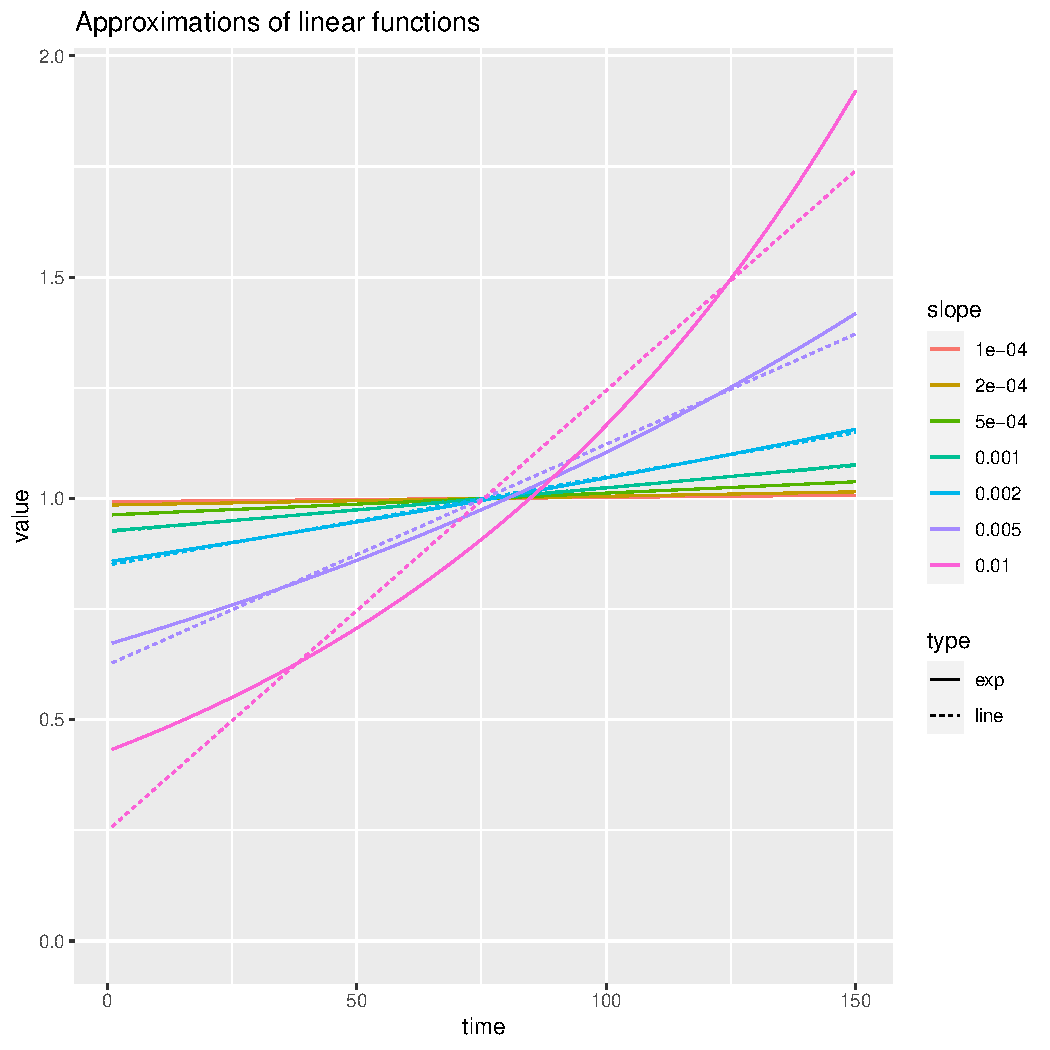
\includegraphics[width=0.7\textwidth]{experiment_3_expline.pdf}
    \end{wrapfigure}
    Длина сигналов $N = 150$
    Функции для сигналов: линейная --- $s^{(i)}_j = slope_i j+(1-slope_i\frac{N}{2})$, экспоненциальная аппроксимация --- $s^{(i)}_j = A \exp(slope_i j)$.

    \note{
        Как видно на графике иногда линейный сигнал можно хорошо аппроксимировать показательной функцией. Причем, качество приближения зависит от угла наклона. Из-за того, что ранг линейного сигнала равен 2, а показательного --- 1, становится интересно, можно ли использовать экспоненциальный сигнал как поддерживающий для линейного?
    }
\end{frame}

% \begin{frame}{Является ли первая компонента разложения линейного ряда показательной функцией?}
%     \begin{figure}[h]
%         \centering
%         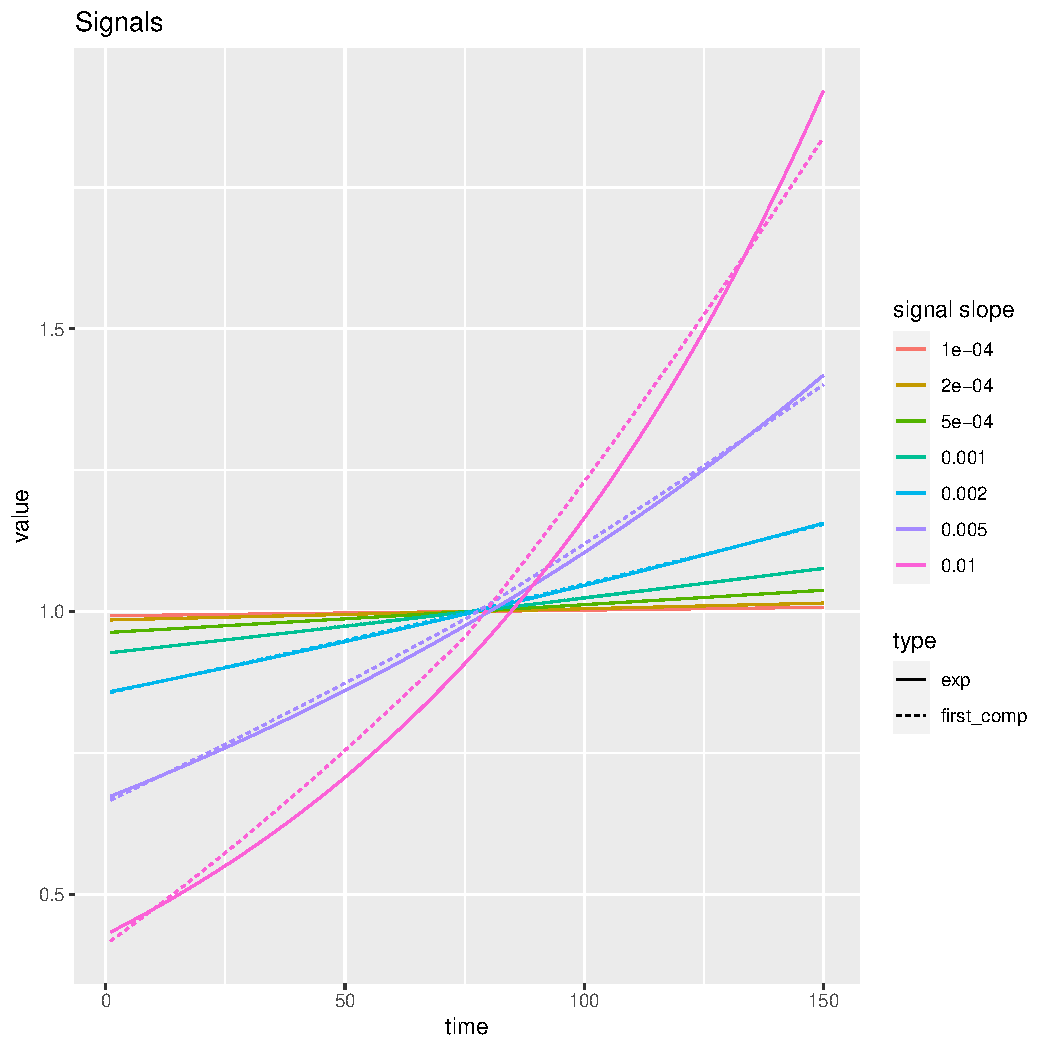
\includegraphics[width=0.7\textwidth]{experiment_3_linefirstcomp.pdf}
%         % \caption{Сравнение первых компонент сигнала и аппроксимирующих экспонент.}
%         % \label{fig:exp3_linefirstcomp}
%     \end{figure}

%     \note{Для того чтобы понять, можно ли использовать экспоненциальный сигнал как поддерживающий для линейного, нужно узнать, насколько их структура похожа. Например, сравнить аппроксимацию линейного сигнала рядом ранга 1 (восстановить первую компоненту алгоритмом $\SSA$) и аппроксимацию этого же сигнала экспоненциальной функцией.
    
%     видно что первая компонента разложения линейного ряда не является показательной функцией, так как показательные функции не могут дважды пересекаться.
%     }
% \end{frame}


% \begin{frame}{Зависимость доли второй компоненты от угла наклона}
%     \begin{figure}[h]
%         \centering
%         \begin{minipage}{.5\textwidth}
%             \centering
%             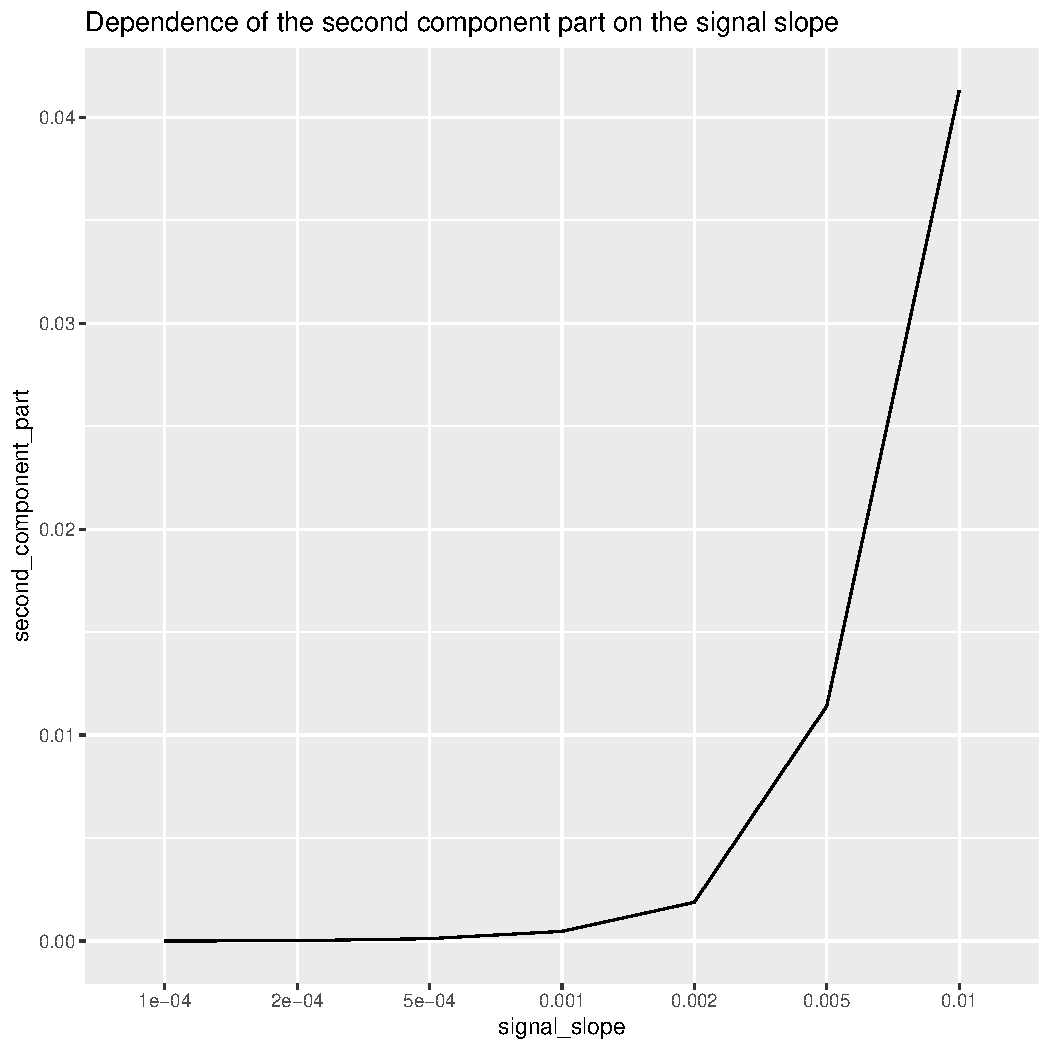
\includegraphics[width=\textwidth]{experiment_3_secondpart1.pdf}
%             % \caption{Зависимость доли второй компоненты от угла наклона линейного сигнала.}
%             % \label{fig:exp3_secondpart1}
%         \end{minipage}%
%         \begin{minipage}{.5\textwidth}
%             \centering
%         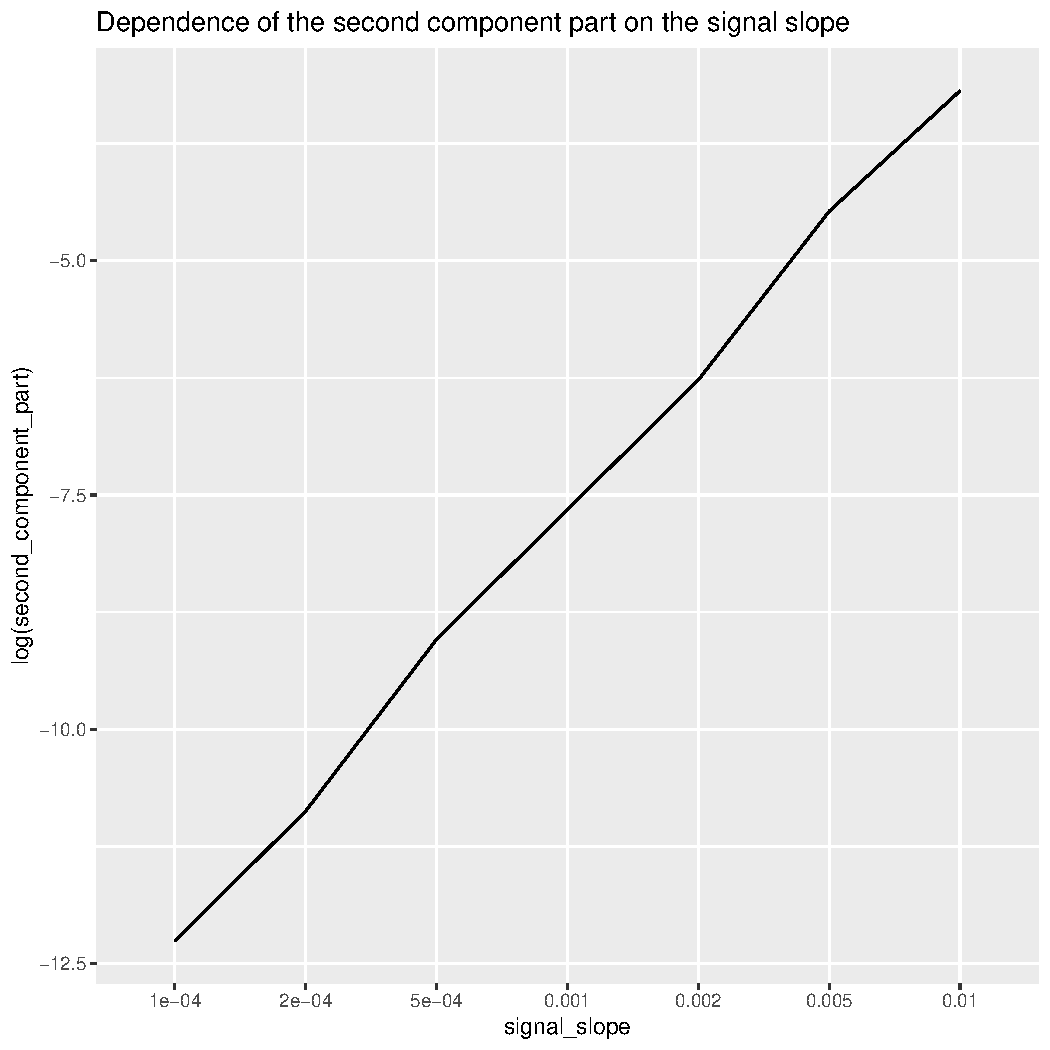
\includegraphics[width=\textwidth]{experiment_3_secondpart2.pdf}
%         % \caption{Зависимость логарифма доли второй компоненты от угла наклона линейного сигнала.}
%         % \label{fig:exp3_secondpart2}
%         \end{minipage}
%     \end{figure}

%     \note{Как уже было замечено, при меньших углах наклона, аппроксимация получается лучше. Есть ли зависимость доли второй компоненты в линейном сигнале от угла наклона?
    
%     На левом зависимость похожа на экспоненциальную, прологарифмируем и проверим это.
%     На правом видна линейная зависимость логарифма доли второй компоненты и угла наклона сигнала, поэтому доля второй компоненты действительно зависит экспоненциально от угла наклона.}
% \end{frame}

% \begin{frame}{При каком шуме вторая компонента теряется}
%     \begin{figure}[h]
%         \centering
%         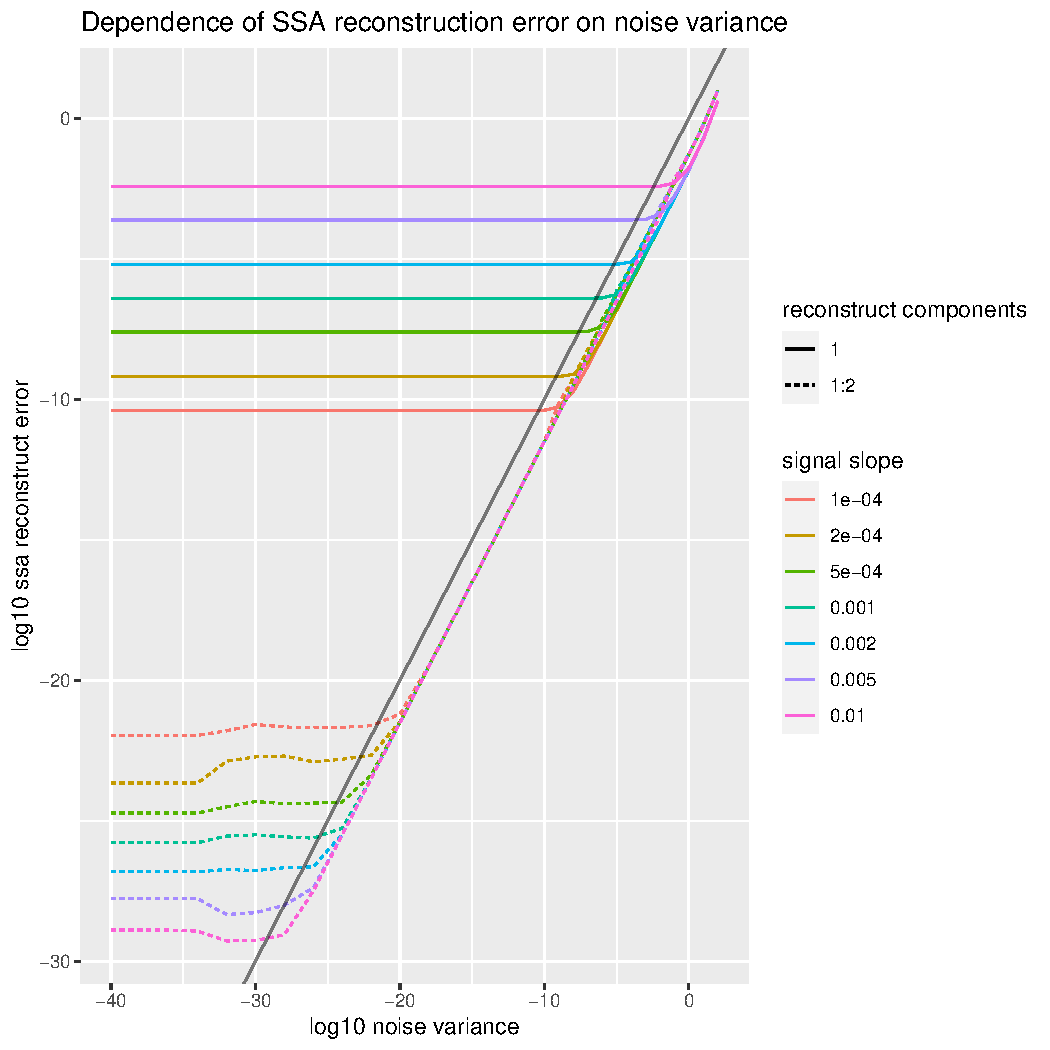
\includegraphics[width=0.7\textwidth]{experiment_3_lost1.pdf}
%         % \caption{Зависимость ошибки восстановления от $\sigma^2$.}
%         % \label{fig:exp3_lost1}
%     \end{figure}

%     \note{На прошлом графике можно заметить, что доля второй компоненты мала, а значит в алгоритме $\SSA$ она может оказаться не второй и быть потеряна при достаточно большом шуме.

%     Как понять, что вторая компонента потерялась не изучая разложение в ручную?
    
%     Будем восстанавливать одну или две компоненты алгоритмом $\SSA$ из линейных сигналов с разными углами наклона и считать ошибку восстановления. Когда вторая компонента теряется, ошибка двух компонент становится больше ошибки одной компоненты, потому что вместо нужной второй компоненты ряда берется часть шума.
    
%     На рис. \ref{fig:exp3_lost1} и \ref{fig:exp3_lost2} черная линия показывает прямую $x = y$, цветные линии --- графики ошибок восстановления, пунктирные --- двумя компонентами, сплошные --- одной. Чтобы ответить на поставленный вопрос, найдем точки пересечения графиков с помощью интерполяции и построим график.}
% \end{frame}

% \begin{frame}{При каком шуме вторая компонента теряется}
%     \begin{figure}[h]
%         \centering
%         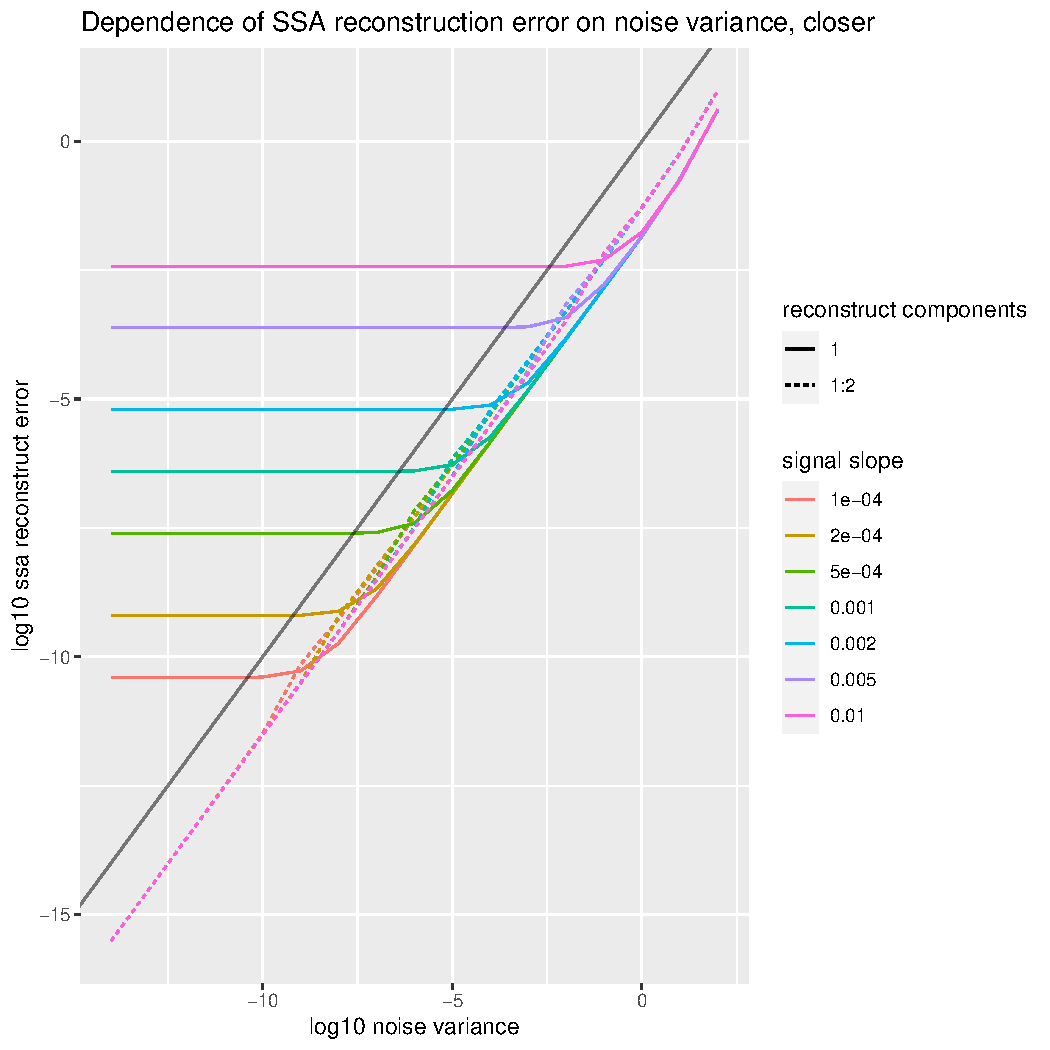
\includegraphics[width=0.7\textwidth]{experiment_3_lost2.pdf}
%         % \caption{Зависимость ошибки восстановления от $\sigma^2$, крупнее.}
%         % \label{fig:exp3_lost2}
%     \end{figure}

%     \note{На прошлом графике можно заметить, что доля второй компоненты мала, а значит в алгоритме $\SSA$ она может оказаться не второй и быть потеряна при достаточно большом шуме.

%     Как понять, что вторая компонента потерялась не изучая разложение в ручную?
    
%     Будем восстанавливать одну или две компоненты алгоритмом $\SSA$ из линейных сигналов с разными углами наклона и считать ошибку восстановления. Когда вторая компонента теряется, ошибка двух компонент становится больше ошибки одной компоненты, потому что вместо нужной второй компоненты ряда берется часть шума.
    
%     На графике черная линия показывает прямую $x = y$, цветные линии --- графики ошибок восстановления, пунктирные --- двумя компонентами, сплошные --- одной. Чтобы ответить на поставленный вопрос, найдем точки пересечения графиков с помощью интерполяции и построим график.}
% \end{frame}

% \begin{frame}{При каком шуме вторая компонента теряется}
%     \begin{figure}[h]
%         \centering
%         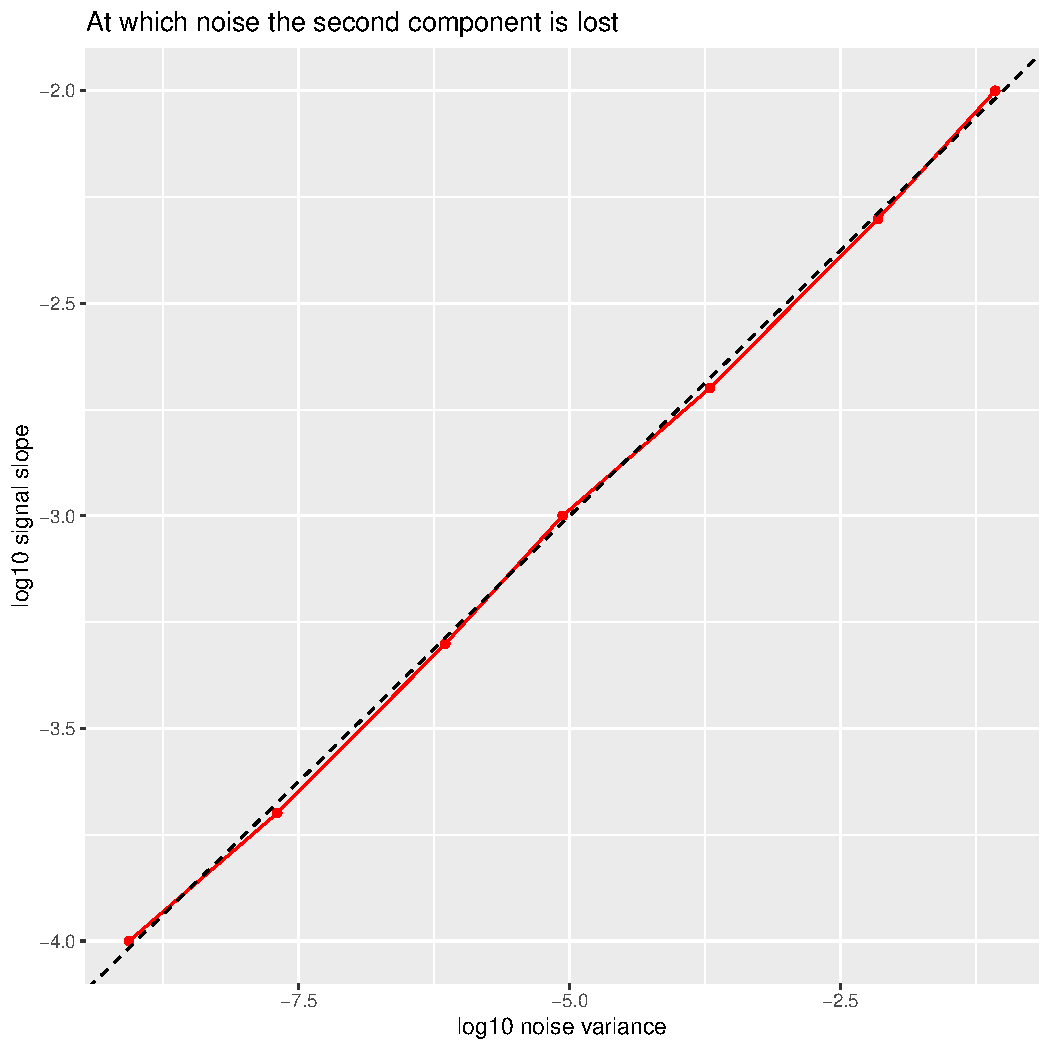
\includegraphics[width=0.7\textwidth]{experiment_3_lost3.pdf}
%         % \caption{Зависимость ошибки восстановления от $\sigma^2$.}
%         % \label{fig:exp3_lost3}
%     \end{figure}

%     \note{На рис. \ref{fig:exp3_lost3} черным пунктиром обозначена прямая $4y = x - 7$. Зависимость логарифмов угла наклона и дисперсии шума близка к уравнению $4\log_{10}(slope) = \log_{10}(\sigma^2) - 7$, поэтому сама зависимость выражается уравнением $slope^4 = 10^{-7}\sigma^2$.}
% \end{frame}

\begin{frame}{Сравнение линейного ряда и его аппроксимации как поддерживающих рядов}
    Длина известного ряда $N=100$. длина прогноза $N_{for} = 20$.
    Функции для сигналов:\\
    линейная --- $s^{(i)}_j = slope_i j+(1-slope_i\frac{N}{2})$,\\
    экспоненциальная аппроксимация --- $A \exp(slope_i j)$.\\
    Сигнал $\sfS^{(1)}$ --- линейный c наклоном $slope_1 \in \{0.0001, 0.01\}$.\\
    Сигналы $\sfS^{(2)}$ --- линейные экспоненциальные c наклонами $slope_2 \in \{0.0001$, $0.0002$, $0.0005$, $0.001$, $0.002$, $0.005$, $0.01\}$.\\
    Шум первого ряда --- аддитивный гауссовский с $\sigma_1 = 0.2$. Второй ряд без шума.
\end{frame}


\begin{frame}{Сравнение линейного ряда и его аппроксимации как поддерживающих рядов}
    \begin{figure}[h]
        \centering
        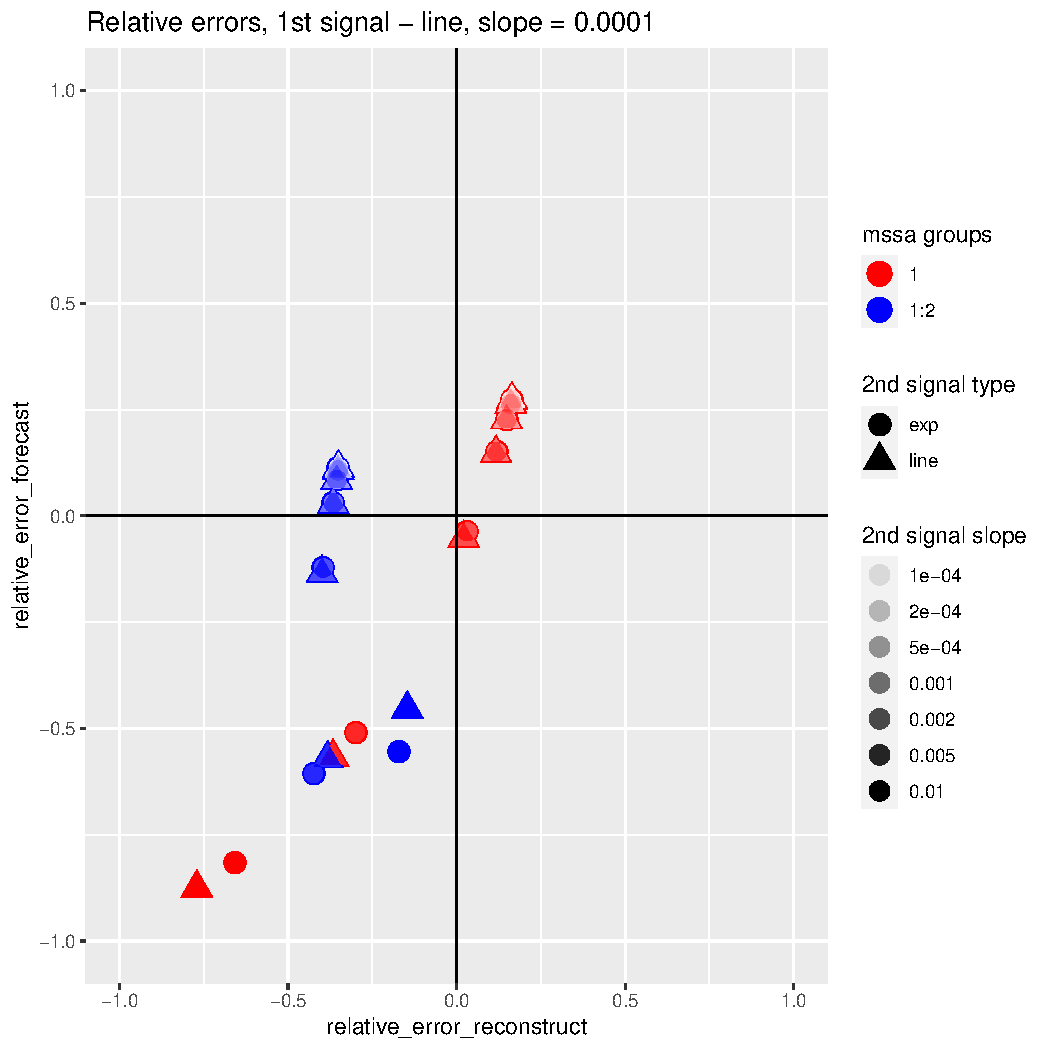
\includegraphics[width=0.65\textwidth]{experiment_3_mssa2.pdf}
        % \caption{Зависимость относительных ошибок от второго ряда и выбора ранга для MSSA, первый сигнал --- линейный с наклоном 0.0001.}
        % \label{fig:exp3_mssa2}
    \end{figure}
    

    \note{
        

        $\MSSA$ хуже $\SSA$ при больших разницах наклона и наоборот для похожих сигналов. Но для восстановления двумя компонентами $\SSA$ всегда лучше. Линейная функция и ее аппроксимация поддерживают примерно одинаково.
    }
\end{frame}

\begin{frame}{Сравнение линейного ряда и его аппроксимации как поддерживающих рядов}
    \begin{figure}[h]
        \centering
        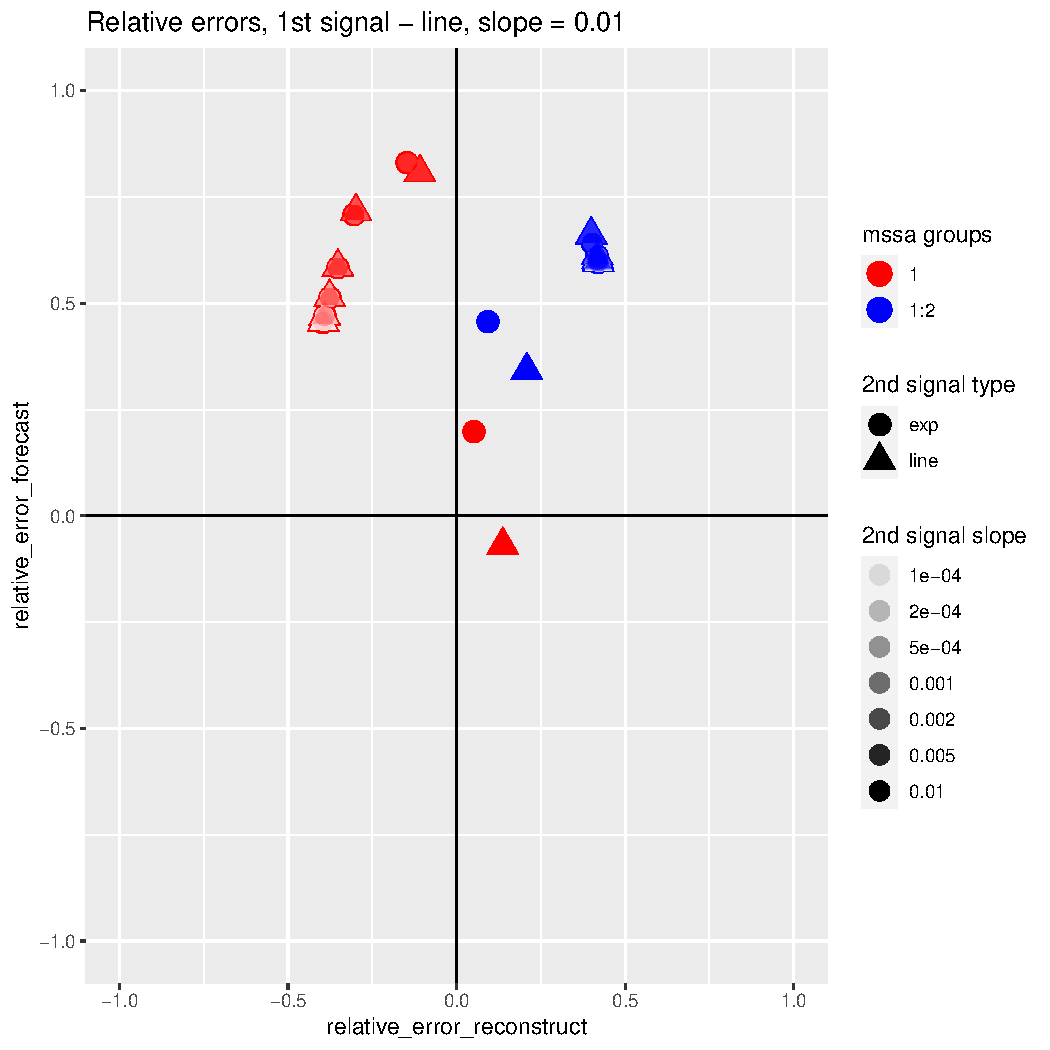
\includegraphics[width=0.65\textwidth]{experiment_3_mssa1.pdf}
        % \caption{Зависимость относительных ошибок от второго ряда и выбора ранга для MSSA, первый сигнал --- линейный с наклоном 0.01.}
        % \label{fig:exp3_mssa1}
    \end{figure}

    \note{На графике при использовании ранга 2 в алгоритме $\MSSA$ ошибка прогноза и восстановления меньше чем $\SSA$ почти для любого второго ряда. Использование ранга 1 может дать еще меньшую ошибку, но редко.}
\end{frame}

\begin{frame}{Результат третьего эксперимента}
    Так как первая компонента разложения линейного ряда оказалась не экспонентой, это значит, что сигналы не полностью согласованы.

    Для линейных функций с большим наклоном алгоритм $\MSSA$ дает результат лучше чем $\SSA$, а маленьким наклоном наоборот.
    
\end{frame}

\begin{frame}{Заключение}
    Найдено много интересных зависимостей.

    Экспоненциальную аппроксимацию линейного ряда можно использовать в качестве поддерживающего ряда для линейных рядов с большим наклоном.

    \note{
        Найдено много интересных зависимостей: линейная зависимость граничного значения среднеквадратичного отклонения и изменения параметра поддерживающего ряда, экспоненциальная зависимость доли второй компоненты в линейном ряду, степенная зависимость дисперсии шума при котором теряется вторая компонента линейного ряда от угла наклона.

        Экспоненциальную аппроксимацию линейного ряда можно использовать в качестве поддерживающего ряда для линейных рядов с большим наклоном.
        еще я придумал как отображать на двумерном графике отношение 4 ошибок, конечно не без потерь информации.
    }
\end{frame}

\begin{frame}{Список литературы}
    \nocite{*}
    \bibliographystyle{ugost2008}
	\bibliography{references}
    % \begin{thebibliography}{3}
    % \bibitem{SSA_with_R}
    % \bibitem{supportive_mssa}
    % \end{thebibliography}    

    \note{
        На данном слайде представлен список основных источников, используемых в моей работе.
    }
\end{frame}

\end{document}
